\documentclass{beamer}
\usepackage{tikz}
\usepackage[orientation=landscape,size=a0,scale=2]{beamerposter}
\usepackage[absolute,overlay]{textpos}
\usetikzlibrary{arrows}
\usetikzlibrary{petri}

\begin{document}

\begin{textblock}{15}(0.5, 0.5)
    \begin{block}{}
        \centering
        \Large Suppression of Variation in Cell-Size: A Control Theoretic Approach \\
        \large Dilawar Singh, \texttt{dilawars@ncbs.res.in}
    \end{block}
    \begin{block}{Abstract}

        We propose a  possible mechanism based on control and information theory
        which can be used to control cell size. We explore few network
        topologies of a simple control network which can keep the size of the
        cell at a fixed value while giving a upper bound on the size of the
        Endosome.

\end{block}
\end{textblock}

\begin{textblock}{7}(0.5,3.5)

    \begin{block}{Network under study}
        \begin{figure}
            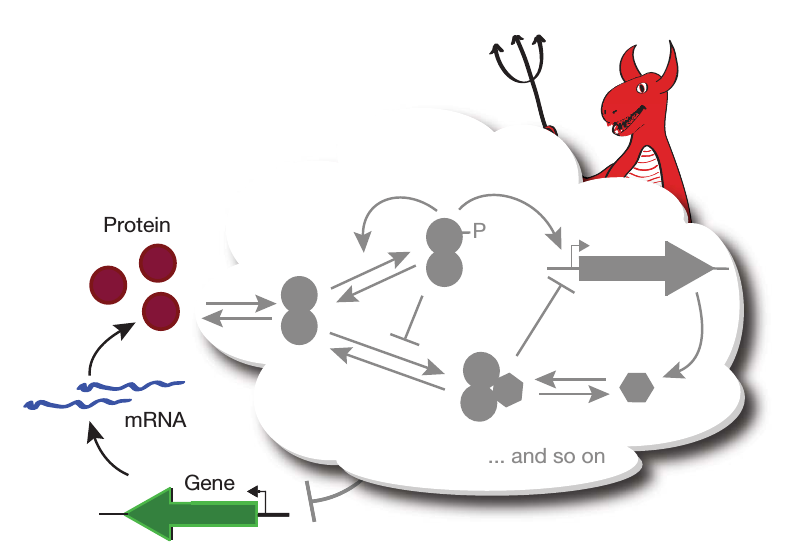
\includegraphics[scale=3]{./fig_mrna_protein.png}
            \begin{tikzpicture}[
                ]
            \node[place,tokens=1,label=above:$X_1$] (X1) at (0,0) {};
            \node[place,colored tokens={red,red,red},label=below:$X_2$] (X2) at (0,-5) {};

            \node[transition,blue,fill,label=above:$f$] (birth) at (3,0) {};
            \node[transition,red,fill,label=below:$\tau$] (death) at (3,-5) {};

            \node[place,label=above:Birth] (Xb) at (10,0) {};
            \node[place,label=below:Death] (Xd) at (10,-5) {};


            \draw[->] (X1) to (birth) to node[above] {\tiny U} (Xb);
            \draw[->] (X1) to  (death);
            \draw[->] (X2) to (death)  to (Xd);
            \draw[->] (X2) to (birth);

            \draw[->,blue] (Xb) to [bend right]  (birth);
            \draw[->,blue] (Xb) to (death);

            \draw[red,->] (Xd) to [bend left] (death) (Xd) to (birth);

            \end{tikzpicture}

        \caption{Network under consideration. In our scheme $x_1$ is mRNA and $x_2$ is protein.}
        \label{fig:demon}
        \end{figure}
    
        \begin{equation}
            %x_1 \rightarrow x_1 + 1 \\
        \end{equation}


    \end{block}

\end{textblock}

\end{document}
